%----------------------------------------------------------------------------------------
%    PACKAGES AND THEMES
%----------------------------------------------------------------------------------------

\documentclass[aspectratio=169,xcolor=dvipsnames]{beamer}
\usetheme{SimplePlus}

\usepackage{graphicx}
\usepackage{hyperref}
\usepackage{booktabs}
\usepackage{tabularx}
\usepackage{array}
\usepackage{tikz}
\usetikzlibrary{arrows.meta,positioning,fit}

\graphicspath{{../figures/}{../../submit_service/app/static/}}

\definecolor{FedctlGreen}{RGB}{73, 154, 136}
\definecolor{FedctlOrange}{RGB}{214, 129, 60}
\definecolor{FedctlPurple}{RGB}{126, 91, 176}
\definecolor{FedctlGray}{RGB}{94, 103, 120}

\newcommand{\smallnote}[1]{{\scriptsize\color{FedctlGray}#1}}
\newcommand{\metric}[2]{\textbf{\large #1}\\[-0.1em]\smallnote{#2}}
\newcommand{\tightitems}{\setlength\itemsep{0.45em}}

%----------------------------------------------------------------------------------------
%    TITLE PAGE
%----------------------------------------------------------------------------------------

\title{\texttt{fedctl}}
\subtitle{A tool for shared realistic edge-FL experiments in Flower}

\author{Samuel Jie}

\institute
{
    Department of Computer Science and Technology \\
    University of Cambridge \\
    % \href{http://fedctl.cl.cam.ac.uk}{\texttt{fedctl.cl.cam.ac.uk}}
}
\date{Flower Monthly \textbar{} 6 May 2026}
\titlegraphic{
\includegraphics[width=0.1\linewidth]{fedctl-circle.png}}

%----------------------------------------------------------------------------------------
%    PRESENTATION SLIDES
%----------------------------------------------------------------------------------------

\begin{document}

\begin{frame}
    \titlepage
\end{frame}

%------------------------------------------------
\section{Why real systems matter}
%------------------------------------------------

\begin{frame}{Federated learning runs on real systems}
    \begin{columns}[T,totalwidth=\textwidth]
        \column{0.54\textwidth}
        \begin{block}{What FL is trying to handle}
            \begin{itemize}
                \tightitems
                \item Data often cannot move because of privacy, governance, bandwidth, or ownership.
                \item The client is a real device, not just a statistical partition.
                \item Availability, CPU speed, memory pressure, and network path become part of training.
            \end{itemize}
        \end{block}

        \column{0.38\textwidth}
        \vspace{0.3em}
        \metric{Same algorithm}{different devices, different timing}

        \vspace{1.2em}
        \metric{Same dataset split}{different update arrival order}

        \vspace{1.2em}
        \metric{Same final accuracy}{different wall-clock cost}
    \end{columns}
\end{frame}

\begin{frame}{Heterogeneity changes the training loop}
    \begin{columns}[T,totalwidth=\textwidth]
        \column{0.47\textwidth}
        \begin{block}{Compute heterogeneity}
            \begin{itemize}
                \tightitems
                \item Devices have different CPU and memory budgets.
                \item Smaller devices may need smaller local models.
                \item The bottleneck shows up as training time and deployed-model quality.
            \end{itemize}
        \end{block}

        \column{0.47\textwidth}
        \begin{exampleblock}{Network and availability}
            \begin{itemize}
                \tightitems
                \item Updates arrive at different times.
                \item Slow clients can contribute less often or with more staleness.
                \item The bottleneck shows up as time-to-target and client influence.
            \end{itemize}
        \end{exampleblock}
    \end{columns}

    \vspace{1.0em}
    \centering
    \textbf{\texttt{fedctl} makes these deployment conditions explicit instead of accidental.}
\end{frame}

\begin{frame}{Simulation hides deployment effects}
    \begin{columns}[T,totalwidth=\textwidth]
        \column{0.47\textwidth}
        \begin{exampleblock}{Convenient simulation}
            \begin{itemize}
                \tightitems
                \item Clients run as local processes.
                \item Timing is either homogeneous or injected as a model.
                \item Failures and logs disappear with the process.
            \end{itemize}
        \end{exampleblock}

        \column{0.47\textwidth}
        \begin{alertblock}{Real edge-style runs}
            \begin{itemize}
                \tightitems
                \item Clients run on different hardware.
                \item Slow devices, bandwidth limits, and queueing are observable.
                \item Every run leaves inspectable evidence.
            \end{itemize}
        \end{alertblock}
    \end{columns}

    \vspace{1.2em}
    \centering
    \textbf{The question becomes: how do we let multiple researchers use this kind of testbed without turning every run into cluster ops?}
\end{frame}

%------------------------------------------------
\section{A shared Raspberry Pi cluster}
%------------------------------------------------

\begin{frame}{A shared Raspberry Pi testbed is feasible}
    \begin{columns}[T,totalwidth=\textwidth]
        \column{0.52\textwidth}
        \begin{tikzpicture}[
            device/.style={draw=DarkBlue!45, rounded corners=2pt, minimum width=0.55cm, minimum height=0.42cm, fill=MutedBlue},
            rpi5/.style={device, fill=FedctlGreen!24},
            rpi4/.style={device, fill=FedctlOrange!24},
            label/.style={font=\scriptsize, text=FedctlGray},
            brace/.style={draw=DarkBlue!55, thick}
        ]
        \node[label, anchor=west] at (-0.1, 2.7) {Current pool: 50 Raspberry Pi workers};
        \foreach \i in {0,...,29} {
            \node[rpi4, minimum width=0.34cm, minimum height=0.26cm] at ({mod(\i,10)*0.42}, {1.75 - floor(\i/10)*0.36}) {};
        }
        \foreach \i in {0,...,19} {
            \node[rpi5, minimum width=0.34cm, minimum height=0.26cm] at ({mod(\i,10)*0.42}, {0.28 - floor(\i/10)*0.36}) {};
        }
        \node[label, anchor=west] at (4.45, 1.38) {\texttt{30 x rpi4}};
        \node[label, anchor=west] at (4.45, 0.02) {\texttt{20 x rpi5}};
        \draw[brace] (-0.25, 1.95) rectangle (4.05, 0.88);
        \draw[brace] (-0.25, 0.48) rectangle (4.05, -0.24);
        \node[label, align=left, anchor=west] at (0.0, -1.10) {Researchers can request the full pool or a typed slice;\\device type is a deployment variable.};
        \end{tikzpicture}

        \column{0.42\textwidth}
        \begin{block}{What is hard}
            \begin{itemize}
                \tightitems
                \item Queueing shared access.
                \item Pinning logical clients to hardware classes.
                \item Repeating runs with the same conditions.
                \item Finding logs and artifacts after something fails.
            \end{itemize}
        \end{block}
    \end{columns}
\end{frame}

\begin{frame}{Submitting Flower projects to the cluster}
    \begin{figure}
        \centering
        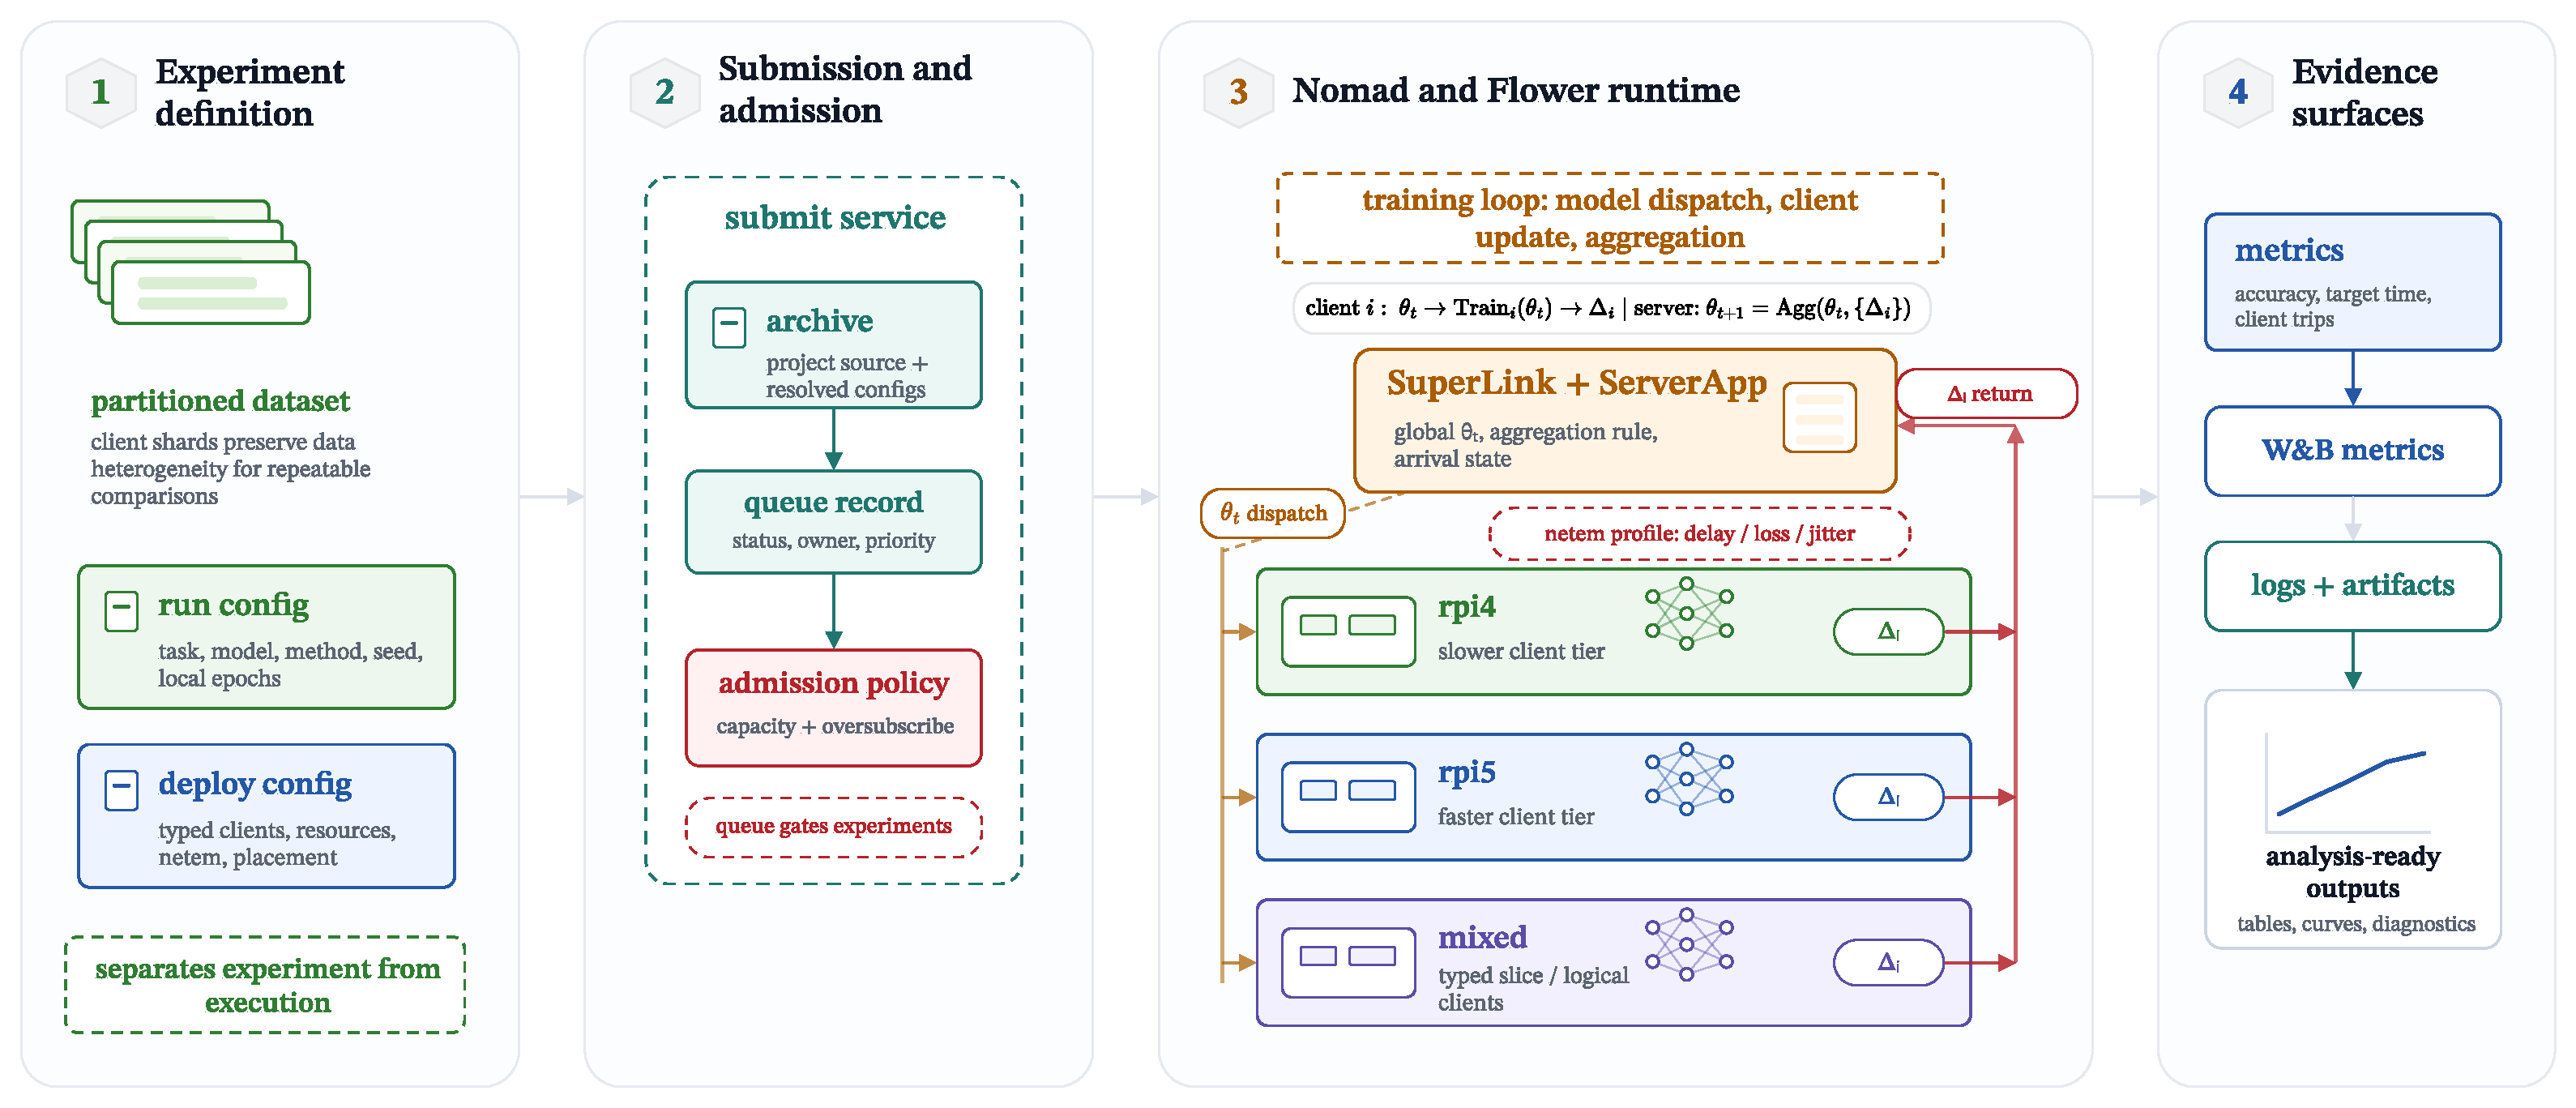
\includegraphics[width=0.95\linewidth]{remote_execution_lifecycle_clean.pdf}
    \end{figure}

    \vspace{-0.6em}
    \begin{columns}[T,totalwidth=\textwidth]
        \column{0.32\textwidth}
        \metric{Submit}{package a Flower project}
        \column{0.32\textwidth}
        \metric{Deploy}{render Nomad jobs and placement}
        \column{0.32\textwidth}
        \metric{Inspect}{logs, jobs, metrics, artifacts}
    \end{columns}
\end{frame}

\begin{frame}{High-level execution stack}
    \centering
    \resizebox{0.93\linewidth}{!}{%
    \begin{tikzpicture}[
      >=Stealth,
      font=\scriptsize,
      arrow/.style={thick, ->},
      infraarrow/.style={thick, ->, dashed},
      coltitle/.style={font=\bfseries\small},
      groupbox/.style={draw, dashed, rounded corners=4pt, minimum width=3.0cm, minimum height=5.10cm, inner sep=0pt},
      cfggroup/.style={groupbox, fill=MutedBlue},
      ctlgroup/.style={groupbox, fill=FedctlGreen!10},
      rungroup/.style={groupbox, fill=FedctlOrange!10},
      obsgroup/.style={groupbox, fill=MutedBlack},
      innerbox/.style={draw, rounded corners=3pt, align=center, text width=2.18cm, minimum height=0.64cm, inner sep=2.5pt},
      cfgbox/.style={innerbox, fill=DarkBlue!16},
      ctlbox/.style={innerbox, fill=FedctlGreen!22},
      runbox/.style={innerbox, fill=FedctlOrange!22},
      obsbox/.style={innerbox, fill=FedctlGray!14},
      basebox/.style={draw, rounded corners=4pt, align=center, fill=white, text width=9.3cm, minimum height=0.76cm, inner sep=5pt}
    ]
    \node[coltitle] at (0.0, 0.35) {Specification};
    \node[coltitle] at (3.55, 0.35) {Control plane};
    \node[coltitle] at (7.10, 0.35) {Flower runtime};
    \node[coltitle] at (10.65, 0.35) {Observability};

    \node[cfggroup] (config) at (0.0, -2.70) {};
    \node[ctlgroup] (control) at (3.55, -2.70) {};
    \node[rungroup] (runtime) at (7.10, -2.70) {};
    \node[obsgroup] (observability) at (10.65, -2.70) {};

    \node[cfgbox, anchor=north] (run) at (0.0, -0.55) {\textbf{Run config}\\Flower choices};
    \node[cfgbox, anchor=north] (dep) at (0.0, -1.85) {\textbf{Deploy config}\\system choices};

    \node[ctlbox, anchor=north] (cli) at (3.55, -0.55) {\textbf{\texttt{fedctl} CLI}\\submit request};
    \node[ctlbox, anchor=north] (svc) at (3.55, -1.45) {\textbf{Submit service}\\queue and auth};
    \node[ctlbox, anchor=north] (reg) at (3.55, -2.35) {\textbf{Registry}\\run image};
    \node[ctlbox, anchor=north] (nomad) at (3.55, -3.25) {\textbf{Nomad renderer}\\jobs / placement};
    \node[ctlbox, anchor=north] (runner) at (3.55, -4.18) {\textbf{Submit runner}\\cluster handoff};

    \node[runbox, anchor=north] (roles) at (7.10, -0.55) {\textbf{Distributed roles}\\SuperLink\\SuperNodes};
    \node[runbox, anchor=north] (app) at (7.10, -1.85) {\textbf{Flower app}\\training code};

    \node[obsbox, anchor=north] (metrics) at (10.65, -0.55) {\textbf{Metrics}\\W\&B summaries};
    \node[obsbox, anchor=north] (art) at (10.65, -1.55) {\textbf{Artifacts}\\results / configs};
    \node[obsbox, anchor=north] (ui) at (10.65, -2.55) {\textbf{UI/logs}\\inspect / debug};

    \node[basebox] (cluster) at (5.35, -6.25) {\textbf{Cluster:} typed Pi workers; Nomad metadata; resources; net profiles};

    \draw[arrow] (config.east) -- (control.west);
    \draw[arrow] (control.east) -- (runtime.west);
    \draw[arrow] (runtime.east) -- (observability.west);
    \draw[infraarrow] (cluster.north) -- ++(0,0.18) -| (control.south);
    \draw[infraarrow] (cluster.north) -- ++(0,0.18) -| (runtime.south);
    \end{tikzpicture}%
    }
\end{frame}

\begin{frame}{Two configs keep the experiment and the system separate}
    \begin{columns}[T,totalwidth=\textwidth]
        \column{0.47\textwidth}
        \begin{block}{Run config}
            \textbf{Flower-facing choices}
            \begin{itemize}
                \tightitems
                \item task, model, data partitioner
                \item method and hyperparameters
                \item client budget, seed, evaluation
            \end{itemize}
        \end{block}

        \column{0.47\textwidth}
        \begin{exampleblock}{Deploy config}
            \textbf{\texttt{fedctl}-facing choices}
            \begin{itemize}
                \tightitems
                \item \texttt{rpi4=30,rpi5=20}
                \item resource and placement policy
                \item network profile and registry
            \end{itemize}
        \end{exampleblock}
    \end{columns}

    \vspace{1.0em}
    \begin{block}{Why this matters}
        The same learning experiment can run on a different topology, and the same topology can run different learning methods.
    \end{block}
\end{frame}

\begin{frame}{Placement and network conditions are explicit}
    \begin{figure}
        \centering
        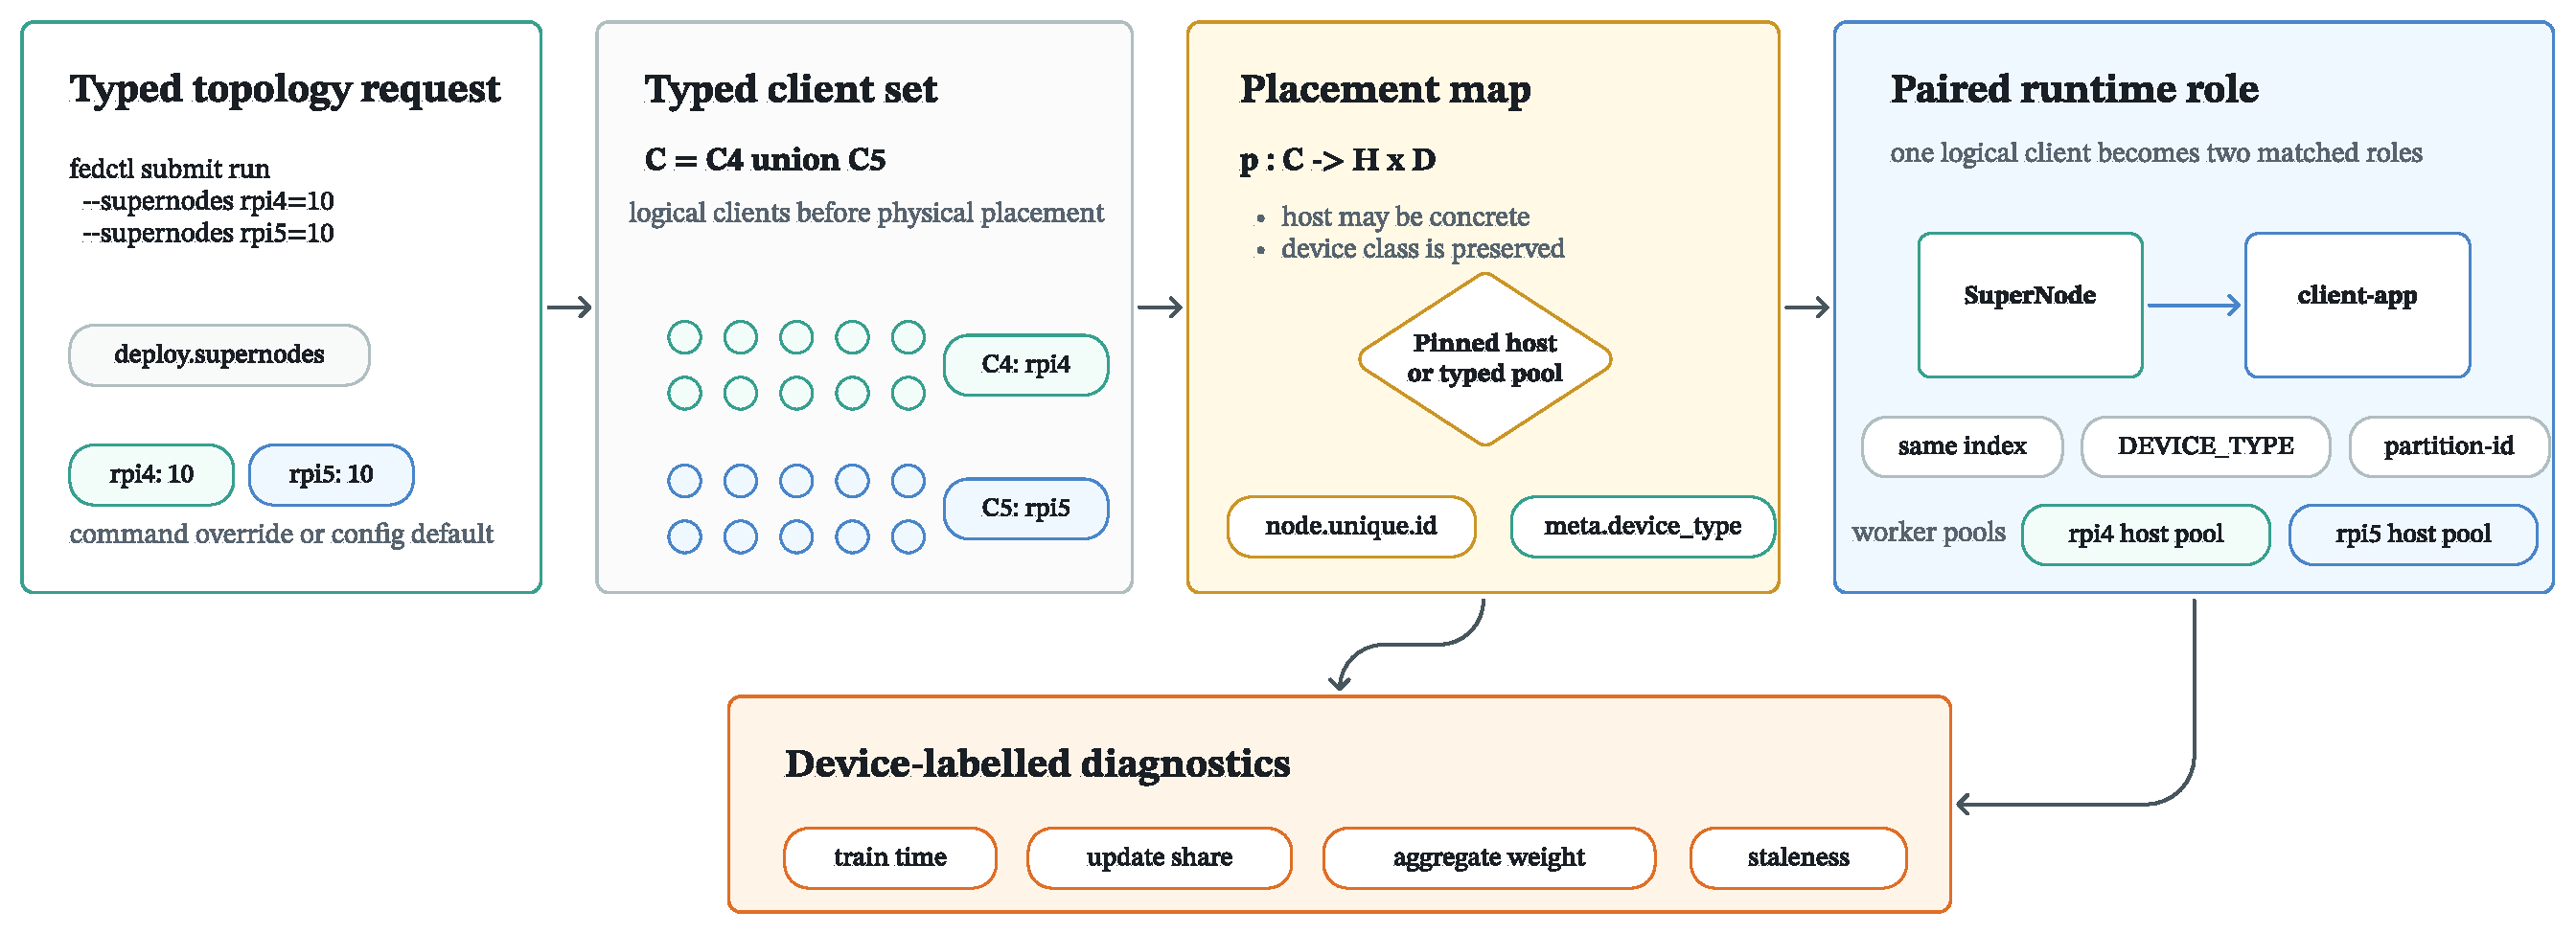
\includegraphics[width=0.88\linewidth]{device_placement_clean.pdf}
    \end{figure}

    \vspace{-0.4em}
    \small
    \begin{tabularx}{\textwidth}{@{}>{\bfseries}p{0.20\textwidth}X@{}}
        Placement & logical clients are mapped onto \texttt{rpi4}/\texttt{rpi5} workers and recorded in metrics. \\
        Network profiles & delay, jitter, loss, and bandwidth caps can be assigned per logical client. \\
    \end{tabularx}
\end{frame}

%------------------------------------------------
\section{Where this is going}
%------------------------------------------------

\begin{frame}{What fedctl makes possible}
    \begin{columns}[T,totalwidth=\textwidth]
        \column{0.31\textwidth}
        \begin{block}{Use real devices}
            \begin{itemize}
                \tightitems
                \item Start from a normal Flower project.
                \item Run on Raspberry Pi workers instead of local processes.
                \item Keep the command-line workflow familiar.
            \end{itemize}
        \end{block}

        \column{0.31\textwidth}
        \begin{exampleblock}{Share the cluster}
            \begin{itemize}
                \tightitems
                \item Queue submissions across users.
                \item Request typed slices from a \(30\) RPi4 + \(20\) RPi5 pool.
                \item Avoid hand-written scheduler jobs.
            \end{itemize}
        \end{exampleblock}

        \column{0.31\textwidth}
        \begin{alertblock}{Change conditions}
            \begin{itemize}
                \tightitems
                \item Fix placement and resources.
                \item Assign network profiles.
                \item Preserve logs, jobs, configs, and artifacts.
            \end{itemize}
        \end{alertblock}
    \end{columns}

    \vspace{0.8em}
    \centering
    \textbf{The useful part is not owning a cluster; it is making it usable as a repeatable Flower workflow.}
\end{frame}

\begin{frame}
    \Huge{\centerline{\textbf{Demo}}}
    \vspace{1.2em}
    \Large{\centerline{\texttt{fedctl submit run ...}}}
    \vspace{0.8em}
    % \large{\centerline{\href{http://fedctl.cl.cam.ac.uk}{\texttt{fedctl.cl.cam.ac.uk}}}}
\end{frame}     

%----------------------------------------------------------------------------------------

\end{document}
